\documentclass[12pt,a4paper]{article}
\usepackage{iftex}
\ifPDFTeX
  \usepackage[T2A]{fontenc}
  \usepackage[utf8]{inputenc}
\else
  \usepackage{fontspec}
  \setmainfont{Liberation Serif}
  \setsansfont{Noto Sans}
  \setmonofont{DejaVu Sans Mono}[Scale=0.84]
\fi
\usepackage[ukrainian]{babel}
\usepackage[a4paper,left=23mm,right=22mm,top=23mm,bottom=24mm]{geometry}
\usepackage{microtype}
\usepackage{setspace}
\setstretch{1.17}
\setlength{\emergencystretch}{3em}
\usepackage{graphicx}
\graphicspath{{./}{screenshots/}}
\usepackage{array,longtable,tabularx,booktabs}
\usepackage{enumitem}
\usepackage{xcolor}
\usepackage{tcolorbox}
\usepackage{tikz}
\usepackage{float}
\usepackage{caption}
\usepackage{fancyhdr}
\usepackage{titlesec}
\usepackage{hyperref}
\usepackage{url}
\usepackage{lastpage}
\usepackage{needspace}
\usepackage{ragged2e}

\newcommand{\AuthorName}{Суворов Дмитро}
\newcommand{\StudentGroup}{ЦІ-31}
\newcommand{\ProjectRepo}{\url{https://github.com/Dima018/Gym_Website}}
\newcommand{\ProjectBoard}{\url{https://github.com/users/Dima018/projects/13}}

\definecolor{forest}{HTML}{233C30}
\definecolor{sage}{HTML}{5B7957}
\definecolor{mist}{HTML}{F0F4EE}
\definecolor{rulegray}{HTML}{D9E1DA}
\hypersetup{hypertexnames=false,colorlinks=true,linkcolor=forest,urlcolor=sage,pdftitle={Звіт КП №2 — сайт спортзалу Ритм},pdfauthor={Суворов Дмитро}}
\titleformat{\section}{\Large\sffamily\bfseries\color{forest}}{\thesection.}{0.6em}{}
\titleformat{\subsection}{\large\sffamily\bfseries\color{forest}}{\thesubsection.}{0.6em}{}
\titlespacing*{\section}{0pt}{15pt}{9pt}
\titlespacing*{\subsection}{0pt}{12pt}{6pt}
\captionsetup{hypcap=false,font=small,labelfont={bf,color=forest},justification=centering}
\setlist[itemize]{leftmargin=1.45em,itemsep=2pt,topsep=4pt}
\setlist[enumerate]{leftmargin=1.55em,itemsep=2pt,topsep=4pt}
\renewcommand{\arraystretch}{1.20}
\pagestyle{fancy}
\fancyhf{}
\fancyhead[L]{\small\sffamily\color{sage} КП №2 · WEB-орієнтовані системи}
\fancyhead[R]{\small\sffamily\color{sage} Ритм}
\fancyfoot[L]{\footnotesize\color{sage} \AuthorName\ · 2026}
\fancyfoot[R]{\footnotesize\color{sage} \thepage\,/\,\pageref{LastPage}}
\renewcommand{\headrulewidth}{0.4pt}
\renewcommand{\headrule}{\hbox to\headwidth{\color{rulegray}\leaders\hrule height \headrulewidth\hfill}}
\setlength{\headheight}{26pt}
\newtcolorbox{infobox}{colback=mist,colframe=rulegray,boxrule=0.5pt,arc=2mm,left=3mm,right=3mm,top=2mm,bottom=2mm}
\newcommand{\file}[1]{\texttt{#1}}
\newcommand{\evidencehead}[2]{%
  \clearpage\subsection*{#1 --- #2}\phantomsection\addcontentsline{toc}{subsection}{#1 --- #2}
}

\newcommand{\shot}[2]{\clearpage\subsection*{#2}\phantomsection\addcontentsline{toc}{subsection}{#2}\begin{center}\includegraphics[width=\linewidth,height=20cm,keepaspectratio]{#1}\end{center}}
\newcommand{\mobiles}[4]{\clearpage\subsection*{Мобільний інтерфейс}\begin{center}\begin{minipage}[t]{.46\linewidth}\centering\includegraphics[width=\linewidth,height=20cm,keepaspectratio]{#1}\\#2\end{minipage}\hfill\begin{minipage}[t]{.46\linewidth}\centering\includegraphics[width=\linewidth,height=20cm,keepaspectratio]{#3}\\#4\end{minipage}\end{center}}

\begin{document}
\begin{titlepage}\thispagestyle{empty}\centering
{\small\sffamily\bfseries МІНІСТЕРСТВО ОСВІТИ І НАУКИ УКРАЇНИ}\par\vspace{5mm}
{\small\sffamily\bfseries НАЦІОНАЛЬНИЙ ТЕХНІЧНИЙ УНІВЕРСИТЕТ УКРАЇНИ}\par
{\small\sffamily\bfseries «КИЇВСЬКИЙ ПОЛІТЕХНІЧНИЙ ІНСТИТУТ ІМЕНІ ІГОРЯ СІКОРСЬКОГО»}\par
\vspace{30mm}{\LARGE\sffamily\bfseries\color{forest} ЗВІТ}\par\vspace{7mm}
{\Large Комп'ютерний практикум №2}\par\vspace{5mm}
{\large «Розробка веб-сайту з базою даних. RESTful API»}\par\vspace{12mm}
з дисципліни\par\medskip
{\large\bfseries «Технології розробки WEB-орієнтованих систем»}\par\vspace{15mm}
\begin{infobox}\centering\large\bfseries Тема №69: «Спортзал»\\Веб-сайт «Ритм»\end{infobox}
\vfill\begin{flushright}Виконавець: \textbf{\AuthorName}\\Група: \StudentGroup\\Викладач: С. В. Суліма\end{flushright}\vfill
Київ --- 2026
\end{titlepage}
\tableofcontents\clearpage
\section{Тема, мета та виконані завдання}
Продовжено проєкт спортзалу «Ритм» з КП №1. Мета роботи --- перейти від статичного сайту до клієнт-серверного застосунку з реляційною базою даних, REST API та автентифікацією.
\begin{itemize}
\item Спроєктовано чотири пов'язані таблиці PostgreSQL та ER-діаграму.
\item Реалізовано Express-сервер, CRUD для тренувань і записів на заняття.
\item Додано реєстрацію, вхід, JWT та розмежування доступу member/admin.
\item Каталог, деталі, форма запису та кабінет інтегровані з API через Fetch.
\item Проведено перевірку API в Insomnia та перевірку клієнта у двох браузерах.
\item Підготовлено документацію API, інструкцію запуску та окремий звіт №2.
\end{itemize}
\noindent\begin{tabularx}{\textwidth}{>{\RaggedRight\arraybackslash\bfseries}p{40mm}X}
Виконавець & \AuthorName\\
Група & \StudentGroup\\
Внесок & Проєктування БД, сервер, клієнтська інтеграція, перевірка і документація\\
\end{tabularx}
Матеріали першої роботи збережено у \file{lab-report/}; нові --- у \file{lab-report-2/}. Статичну версію позначено Git-тегом \file{lab1-v1.0}.

\section{База даних}
\subsection{Сутності, атрибути та зв'язки}
\begin{longtable}{>{\RaggedRight\arraybackslash}p{29mm}>{\RaggedRight\arraybackslash}p{72mm}>{\RaggedRight\arraybackslash}p{51mm}}
\toprule Таблиця & Основні атрибути & Ключі\\\midrule
users & id, name, email, password\_hash, role, created\_at & PK id; UNIQUE email\\
categories & id, name & PK id; UNIQUE name\\
trainings & id, category\_id, name, description, duration\_minutes, price\_cents, image, created\_at & PK id; FK category\_id; UNIQUE name\\
bookings & id, user\_id, training\_id, session\_date, phone, note, created\_at & PK id; FK user\_id, training\_id; UNIQUE(user\_id, training\_id, session\_date)\\\bottomrule
\end{longtable}
Категорія має багато тренувань; користувач має багато записів; тренування має багато записів. Усі зовнішні ключі мають \file{ON DELETE RESTRICT}. Неможливо видалити тренування, доки на нього існують записи. Дублювання запису на ту саму дату обмежено складеним унікальним ключем.

Ціна зберігається цілими копійками, тривалість --- хвилинами, дата заняття --- типом \file{date}, час створення --- \file{timestamptz}. Поля обов'язкові; коментар може бути порожнім рядком. CHECK обмежує роль, тривалість, ціну, формат телефону й дозволені зображення.

\subsection{Обґрунтування третьої нормальної форми}
Усі атрибути атомарні (1НФ). Неключові атрибути повністю залежать від первинного ключа, часткових залежностей немає (2НФ). Назви категорій, імена користувачів та назви/ціни тренувань не дублюються у залежних таблицях: API отримує їх через JOIN. Транзитивних залежностей неключових атрибутів немає (3НФ). Телефон належить конкретному запису і може відрізнятися між записами одного користувача.

\clearpage\subsection{ER-діаграма}
\begin{center}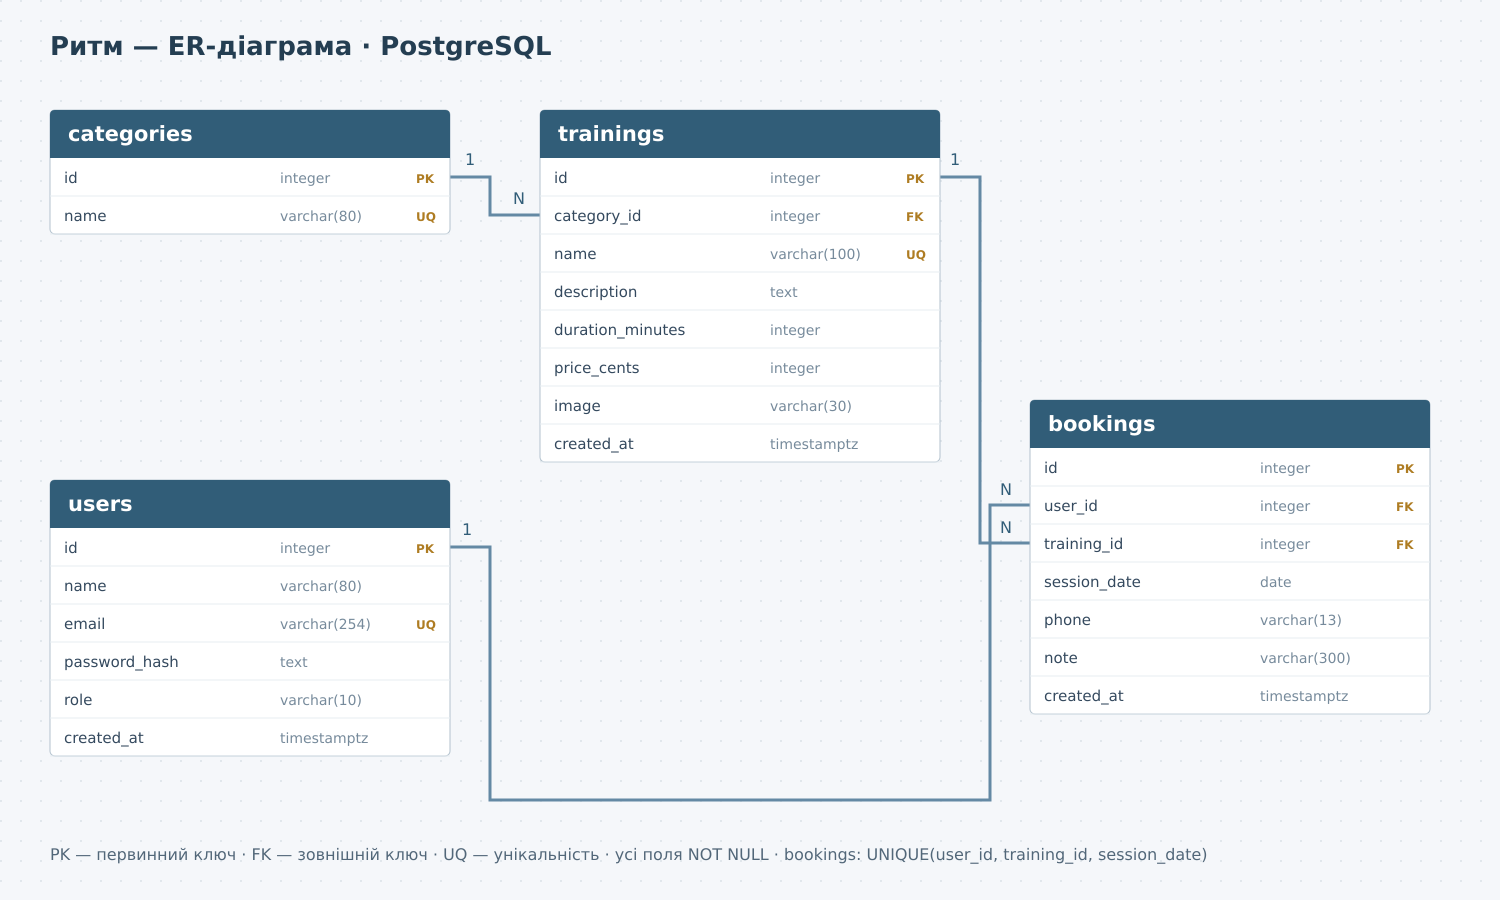
\includegraphics[width=\linewidth]{er-diagram.png}\end{center}
На діаграмі наведено поля, типи й зв'язки 1:N. Модель \file{database/schema.dbml} можна імпортувати у dbdiagram.io; виконувана схема з обмеженнями міститься у \file{database/schema.sql}.

\section{Архітектура та запуск}
Стек: Node.js 22+, Express 5, PostgreSQL 17, драйвер \file{pg}, Zod, bcryptjs, jsonwebtoken, Helmet. Сервер одночасно роздає дозволені HTML/CSS/JS/PNG/WOFF2 та API на одному origin. Клієнт не має прямого доступу до БД.
\begin{center}\begin{tikzpicture}[every node/.style={draw=rulegray,fill=mist,rounded corners,align=center,font=\small,minimum height=12mm}]
\node (a) at (0,0) {Браузер\\HTML/CSS/Fetch};\node (b) at (5,0) {Express\\JSON / JWT / Zod};\node (c) at (10,0) {PostgreSQL\\4 таблиці};\draw[->,thick] (a)--(b);\draw[->,thick] (b)--(c);
\end{tikzpicture}\end{center}
\begin{itemize}
\item \file{server/index.js}: маршрути, автентифікація, права доступу, валідація та обробник помилок.
\item \file{server/db.js}: пул з'єднань і параметризовані SQL-запити.
\item \file{scripts/setup.js}: створення локальних випадкових секретів.
\item \file{scripts/init-db.js}: схема, початкові категорії, шість тренувань і адміністратор.
\item \file{scripts/api.js}: Fetch, Bearer JWT, таймаут, обробка 401 і мережевих помилок.
\item \file{scripts/app.js}: каталог, деталі, кабінет, форма та редактор адміністратора.
\end{itemize}
Порядок запуску:
\begin{verbatim}
npm ci
npm run setup
docker compose up -d --wait db
npm run db:init
npm start
\end{verbatim}
Адреса: \url{http://localhost:3000}. Пароль адміністратора та секрети зберігаються тільки в локальному \file{.env}, виключеному з Git. Звичайний користувач реєструється у кабінеті. PostgreSQL зберігає дані у Docker volume, тому перезапуск не видаляє записи.

\section{REST API}
API використовує ресурсні URL, методи GET/POST/PATCH/DELETE та JSON. Тренування підтримують повний CRUD; записи також підтримують повний CRUD з перевіркою власника. Категорії доступні для читання.
\begin{longtable}{>{\RaggedRight\arraybackslash}p{20mm}>{\RaggedRight\arraybackslash}p{50mm}>{\RaggedRight\arraybackslash}p{31mm}>{\RaggedRight\arraybackslash}p{45mm}}
\toprule Метод & URL (префікс /api) & Доступ & Результат\\\midrule
GET & /health & усі & 200: БД доступна\\
POST & /auth/register & усі & 201: user, token\\
POST & /auth/login & усі & 200: user, token\\
GET & /auth/me & JWT & 200: профіль\\
GET & /categories & усі & 200: список\\
GET & /trainings & усі & 200: каталог\\
GET & /trainings/:id & усі & 200: тренування\\
POST & /trainings & admin & 201 + Location\\
PATCH & /trainings/:id & admin & 200: оновлення\\
DELETE & /trainings/:id & admin & 204: без тіла\\
GET & /bookings & JWT & 200: власні записи\\
GET & /bookings/:id & власник & 200: запис\\
POST & /bookings & JWT & 201 + Location\\
PATCH & /bookings/:id & власник & 200: оновлення\\
DELETE & /bookings/:id & власник & 204: без тіла\\\bottomrule
\end{longtable}
\subsection{Приклади запитів і відповідей}
Реєстрація:
\begin{verbatim}
POST /api/auth/register
{"name":"Dmytro","email":"dmytro@example.com",
 "password":"Example-Password-123"}
201 Created
{"user":{"id":2,"name":"Dmytro",
 "email":"dmytro@example.com","role":"member"},
 "token":"<JWT>","expires_in":3600}
\end{verbatim}
Створення тренування (admin):
\begin{verbatim}
POST /api/trainings
{"category_id":1,"name":"Functional training",
 "description":"Training with an instructor.",
 "duration_minutes":50,"price_cents":35000,
 "image":"personal.png"}
201 Created
Location: /api/trainings/8
{"data":{"id":8,"category_id":1,
 "name":"Functional training",
 "description":"Training with an instructor.",
 "duration_minutes":50,"price_cents":35000,
 "image":"personal.png","created_at":"..."}}
PATCH /api/trainings/8
{"price_cents":36000}
200 OK
DELETE /api/trainings/8
204 No Content
\end{verbatim}
Створення запису (дата повинна бути актуальною):
\begin{verbatim}
POST /api/bookings
{"training_id":1,"session_date":"2026-11-20",
 "phone":"+380671234567","note":"First session"}
201 Created
{"data":{"id":4,"user_id":2,"training_id":1,
 "session_date":"2026-11-20","phone":"+380671234567",
 "note":"First session","created_at":"...",
 "training_name":"...","price_cents":25000,
 "duration_minutes":60}}
PATCH /api/bookings/4
{"note":"Updated note"}
200 OK
DELETE /api/bookings/4
204 No Content
\end{verbatim}
Повні приклади, параметри, коди помилок та імпортована колекція наведені у \file{docs/API.md} і \file{docs/insomnia-collection.json}.

\subsection{Валідація та обробка помилок}
Сервер перевіряє типи, обов'язкові поля й межі; невідомі поля та порожній PATCH відхиляються. Пароль: мінімум 12 символів, максимум 72 UTF-8 байти. Назва тренування: 2--100 символів; опис: 10--2000; тривалість: 15--240 хв; ціна: 0--1000000 копійок. Для запису перевіряються календарна дата від сьогодні до року вперед, телефон формату +380 та дев'ять цифр, коментар до 300 символів.

400 означає некоректні вхідні дані; 401 --- відсутню/невдалу автентифікацію; 403 --- недостатні права; 404 --- відсутній або чужий ресурс; 409 --- конфлікт унікальності чи зовнішнього ключа; 500 --- внутрішню помилку. SQL і стек помилки не передаються клієнту. Повідомлення містить загальне пояснення та, для валідації, масив помилок полів.

\section{Автентифікація та авторизація}
Після реєстрації пароль хешується bcrypt з cost 12, зберігається тільки password\_hash. Email нормалізується до нижнього регістру. Реєстрація не дозволяє призначити собі роль admin.

Після входу сервер видає JWT HS256 із subject, issuer, audience та строком дії одна година. Клієнт зберігає токен у sessionStorage і надсилає його в Authorization: Bearer. Сервер перевіряє підпис, строк, issuer/audience та актуального користувача. Таблиця сесій не ведеться: кожен запит самодостатній. Вихід видаляє токен з браузера; виданий токен залишається чинним до завершення строку дії.

Каталог змінює тільки admin. У SQL-запитах до bookings одночасно перевіряються id ресурсу та user\_id з перевіреного токена. Чужий запис повертає 404. Додаткові заходи: параметризовані SQL-запити, Helmet/CSP, обмеження тіла JSON до 16 КБ та rate limit для входу/реєстрації. Для розгортання в інтернеті потрібен HTTPS.

\section{Перевірка API та інтеграції}
Запити виконано у Insomnia Local Vault. Перевірено GET каталогу, створення, редагування та видалення тренувань і записів та негативні відповіді 400, 401, 403 і 404. Скриншоти фактичних відповідей наведено нижче. Додаткові перевірочні HTTP-запити підтвердили 409 при дублюванні, обмеження FK та ізоляцію записів різних користувачів. Журнал 27 сценаріїв: \file{api-verification.json}. Це перевірка під час розроблення; окремі автоматизовані unit/API-набори КП №3 ще не реалізовувалися.

Клієнт перевірено у Chromium та Firefox при ширинах 390 і 1440 px. Підтверджено завантаження даних, зображень, вхід, керування своїми записами, адміністративний CRUD, повідомлення про помилку мережі та повторне завантаження. Скриншоти відображають дані реальної локальної PostgreSQL-бази. Початкові шість тренувань створені seed-скриптом.

\shot{insomnia-catalog.png}{GET: каталог із PostgreSQL}

\shot{insomnia-create-training.png}{POST: створення тренування, 201}

\shot{insomnia-update-training.png}{PATCH: зміна тренування, 200}

\shot{insomnia-create-booking.png}{POST: створення запису, 201}

\shot{insomnia-update-booking.png}{PATCH: зміна запису, 200}

\shot{insomnia-delete-booking.png}{DELETE: видалення запису, 204}

\shot{insomnia-delete-training.png}{DELETE: видалення тренування, 204}

\shot{insomnia-validation.png}{Валідація: некоректна ціна, 400}

\shot{insomnia-unauthorized.png}{Без токена: 401}

\shot{insomnia-forbidden.png}{Недостатні права: 403}

\shot{insomnia-not-found.png}{Відсутній ресурс: 404}
\clearpage\section{Оновлений клієнтський інтерфейс}
\shot{desktop-trainings.png}{Каталог із бази даних}

\shot{desktop-strength-training.png}{Деталі тренування}

\shot{desktop-auth.png}{Реєстрація та вхід}

\shot{desktop-training-signup.png}{Форма запису на заняття}

\shot{desktop-account.png}{Кабінет із власними записами}

\shot{desktop-admin.png}{Керування каталогом}

\shot{network-error.png}{Помилка мережі та повторний запит}

\mobiles{mobile-trainings.png}{Каталог}{mobile-account.png}{Кабінет}
\mobiles{mobile-training-signup.png}{Форма запису}{mobile-admin.png}{Адміністратор}
\clearpage\section{Висновки}
Статичний сайт КП №1 розширено до клієнт-серверного застосунку. Реалізовано чотири пов'язані таблиці у 3НФ, REST CRUD двох основних сутностей, реєстрацію та вхід із bcrypt/JWT, перевірку власника й ролей. Клієнт працює з даними через Fetch, показує стани завантаження та помилок. API перевірено через Insomnia, інтерфейс --- у двох браузерах. Підготовлено SQL/DBML, документацію API та відтворювану інструкцію запуску. Матеріали КП №1 збережено окремо для демонстрації розвитку проєкту.

\section{Посилання та матеріали}
\begin{itemize}
\item Репозиторій: \ProjectRepo.
\item Дошка задач: \ProjectBoard.
\item Документація Express: \url{https://expressjs.com/en/guide/error-handling.html}.
\item Параметризовані запити pg: \url{https://node-postgres.com/features/queries}.
\item ER-модель для імпорту: \file{database/schema.dbml}.
\item Інструкція ручної перевірки: \file{docs/API.md}.
\end{itemize}
\end{document}
